\documentclass[a4paper, titlepage]{article}
\title{Sobre cubrices y resultados de la extrapolación matricial.}
\author{Erik López de la Fuente}
\date{\today}

\usepackage[table]{xcolor}
\usepackage[utf8]{inputenc}
\usepackage[spanish]{babel}
\usepackage{amsmath}
\usepackage{amsfonts}
\usepackage{enumerate}
\usepackage{graphicx}
\usepackage{float}
\usepackage{makecell}
\usepackage{hyperref}
\usepackage{listings}

\counterwithin*{equation}{section}
\counterwithin*{equation}{subsection}
\counterwithin*{equation}{subsubsection}

\begin{document}

\maketitle

\begin{abstract}
	Una exploración sobre cómo extrapolar el concepto de matriz a la tercera dimensión (\textit{cubriz}), con el correspondiente análisis de sus propiedades y nociones básicas (producto, par identidad, par inverso, representación gráfica...).
\end{abstract}

\tableofcontents
\newpage

\section{Introduction.} \label{intro}

The concept of matrices is, without a doubt, inseparable from linear algebra, as it constitutes a fundamental structure in physics, computer science, artificial intelligence and many more fields of knowledge.

The root of this relevance lies on how simple it makes working with large datasets when processing information, for example, via matrix multiplication.

In this brief article we will investigate a possible way of extrapolating this concept into higher dimensions. In this task we'll find ourselves needing to define a more general notion of a \textit{product}, which will carry problems like the existance of \textit{non-unique identity elements} and the need to develop a theory on the meaning of \textit{inverse elements}.

In this article we'll focus on the three-dimensional particular case (whose elements we'll call ``cubrices''). Having studied cubrices' behaviour, it'll be possible to extrapolate the idea to n dimensions in the future.

This theoretical exercise doesn't aspire to find great use cases to these mathematical objects, but to explore human thought structure's borders. Despite that, we're sure that they may be convenient in some context.
            % Cojonudo
\section{Definiciones.} \label{defs}

\subsection{La estructura del $\mathbb{K}$-álgebra $M_n (\mathbb{K})$.} \label{defs-structure}

%Definimos $M_{m\times n\times o} (\mathbb{K}) = \{ [\mu_{ijk}] \in \mathbb{K}, 1 \le i,j,k; i \le m, j \le n, k \le o\}$ como el conjunto de las \textit{cubrices} y $M_n (\mathbb{K}) = M_{n\times n\times n} (\mathbb{K})$ como el conjunto de las \textit{cubrices cúbicas}. Por convención, una cubriz se representa con una letra griega mayúscula ($A, B, \Gamma, \Delta \in M_{m\times n\times o}$) y sus elementos se representan con letras griegas mayúsculas o minúsculas y su respectivo subíndice ($A_{ijk} = \alpha_{ijk}, B_{ijk} = \beta_{ijk}, \Gamma_{ijk} = \gamma_{ijk}, \Delta_{ijk} = \delta_{ijk}$).

Definimos $M_{m\times n\times o} (\mathbb{K}) = \{ [\mu_{ijk}] \in \mathbb{K}, 1 \le i \le m, 1 \le j \le n, 1 \le k \le o\}$ como el conjunto de las \textit{cubrices} y $M_n (\mathbb{K}) = M_{n\times n\times n} (\mathbb{K})$ como el conjunto de las \textit{cubrices cúbicas}. Por convención, una cubriz se representa con una letra griega mayúscula ($A, B, \Gamma, \Delta \in M_{m\times n\times o}$) y sus elementos se representan con letras griegas mayúsculas o minúsculas y su respectivo subíndice ($A_{ijk} = \alpha_{ijk}, B_{ijk} = \beta_{ijk}, \Gamma_{ijk} = \gamma_{ijk}, \Delta_{ijk} = \delta_{ijk}$).

%Sea $M_{m\times n\times o} (\mathbb{K}) = \{ [\mu_{ijk}] \in \mathbb{K}, 1 \le i,j,k \le m,n,o\}$ 

Podemos definir dos operaciones:

\begin{itemize}
	\item Suma de cubrices. $+: M_{m\times n\times o} \times M_{m\times n\times o} \rightarrow M_{m\times n\times o}, (A, B) \mapsto \Gamma$ tal que $\Gamma_{ijk} = A_{ijk} + B_{ijk}$.
	\item Producto por un escalar. $\cdot: \mathbb{K} \times M_{m\times n\times o} \rightarrow M_{m\times n\times o}, (a, A) \mapsto B$ tal que $B_{ijk} = a \cdot A_{ijk}$.
\end{itemize}

Si $\mathbb{K}$ es un anillo, la n-upla $M_n (\mathbb{K}) = (M_n, \mathbb{K}, +, \cdot)$ es un $\mathbb{K}$-módulo. Si $\mathbb{K}$ es además un cuerpo, $M_n (\mathbb{K})$ será un $\mathbb{K}$-espacio vectorial.

\newpage

Tenemos ahora la suficiente infraestructura para definir el \textit{producto entre cubrices}:

$$\cdot: M_{m\times n\times o} (\mathbb{K}) \times M_{p\times q\times r} (\mathbb{K}) \times M_{s\times t\times u} (\mathbb{K}) \rightarrow M_{v\times w\times x} (\mathbb{K}), (A, B, \Gamma) \mapsto \Delta$$ tal que se cumpla que:

\begin{itemize}
	\item $\Delta_{ijk} = \sum\limits_{l=1}^{n} A_{ilk} \cdot B_{ljk} \cdot \Gamma_{ijl}$.
	\item $n = p = u$.
	\item $v = \min\{m, s\}$.
	\item $w = \min\{q, t\}$.
	\item $x = \min\{o, r\}$.
\end{itemize}

Por supuesto, la n-upla $M_n (\mathbb{K}) = (M_n, \mathbb{K}, \cdot)$ es un $\mathbb{K}$-álgebra.

\subsection{Propiedades de las cubrices.} \label{defs-properties}

Resulta trivial demostrar las siguientes propiedades:

\begin{itemize}
	\item Conmutatividad de la suma: $A + B = B + A$.
	\item Asociatividad de la suma: $(A + B) + \Gamma = A + (B + \Gamma)$.
	\item Asociatividad del producto por un escalar: $a\cdot (b\cdot A) = (a\cdot b)A$.
	\item Conmutatividad del producto por un escalar: $a\cdot (b\cdot A) = b\cdot (a\cdot A)$.
	\item Distributividad del escalar: $a\cdot (A + B) = a\cdot A + a\cdot B$.
	\item Distributividad de la cubriz: $(a + b)\cdot A = a\cdot A + b\cdot A$.
	\item Asociatividad del producto cubriz: $(A \cdot B \cdot \Gamma) \cdot \Delta \cdot E = A \cdot (B \cdot \Gamma \cdot \Delta) \cdot E = A \cdot B \cdot (\Gamma \cdot \Delta \cdot E)$.
	\item Existencia de una \textit{cubriz nula}: $0_{ijk} = 0$.
	\item Existencia de \textit{cubrices opuestas}: $A + (-A) = 0 \Leftrightarrow (-A)_{ijk} = -(A_{ijk}) \forall A$.
\end{itemize}

Gracias a las propiedades asociativas podemos omitir el uso de paréntesis por comodidad. Por ejemplo, $A \cdot (B \cdot \Gamma \cdot \Delta) \cdot E = A \cdot B \cdot \Gamma \cdot \Delta \cdot E$. Omitiremos también el símbolo del producto: $(a\cdot b)\cdot (A \cdot B \cdot \Gamma) = (ab)(AB\Gamma)$.

Es notable la ausencia de una noción de \textit{cubriz identidad} y otra de \textit{cubriz inversa}. Estos conceptos están sujetos a ciertas sutilezas, por lo que antes de explorarlos nos aseguraremos de haber obtenido una buena intuición sobre la apariencia de las cubrices y sus operaciones.
      % Cojonudo
\section{Representaciones gráficas.}

\subsection{Bidimensional.}

Podemos representar cualquier cubriz como una serie de matrices separadas por barras verticales, donde cada matriz sería una ``rodaja'' ($k=1$, $k=2$...) de la cubriz. Esta es la representación estándar para imprenta.

\[ \left(
\begin{array}{c c c | c | c c c}
	\alpha_{111} & \cdots & \alpha_{1n1} &        & \alpha_{11o} & \cdots & \alpha_{1no} \\
	\vdots       &        & \vdots       & \cdots & \vdots       &        & \vdots       \\
	\alpha_{m11} & \cdots & \alpha_{mn1} &        & \alpha_{m1o} & \cdots & \alpha_{mno} \\
\end{array} \right)
\]

\subsection{Tridimensional superficial.}

En ocasiones bastará con una vista panorámica de la cubriz que no entre en detalle. Para este fin podemos organizar cada elemento en vóxeles que constituyan un prisma rectangular.

\begin{figure}[H]
	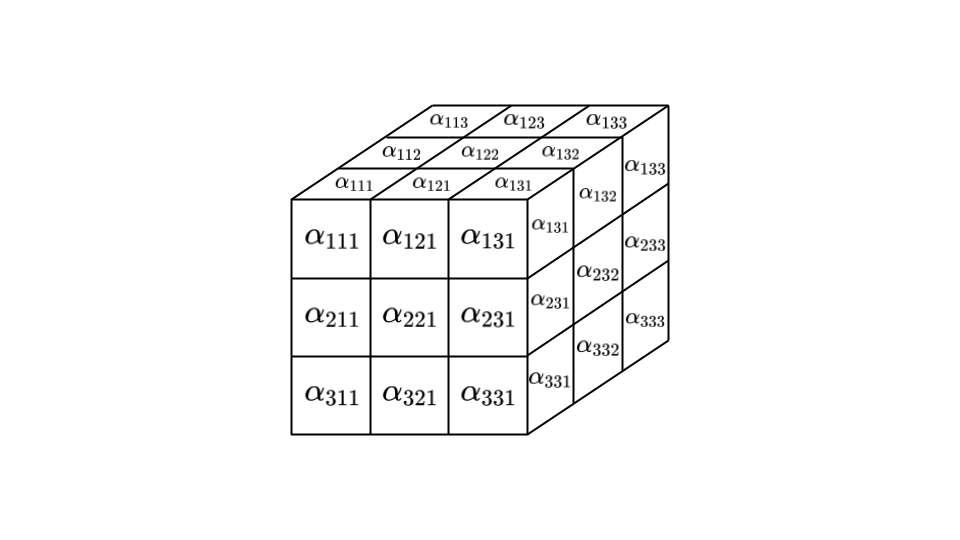
\includegraphics[width=\linewidth]{media/tridimensional_sup.png}
	\caption{Representación tridimensional superficial de una cubriz con elementos $\alpha_{ijk}$.}
\end{figure}

\newpage

\subsection{Tridimensional completa.}

Para una vista completa pero que conserve la estructura tridimensional, podemos separar cada ``rodaja'' de la cubriz a lo largo de un subíndice. Esta representación puede asistir en el reconocimiento de patrones.

\begin{figure}[H]
	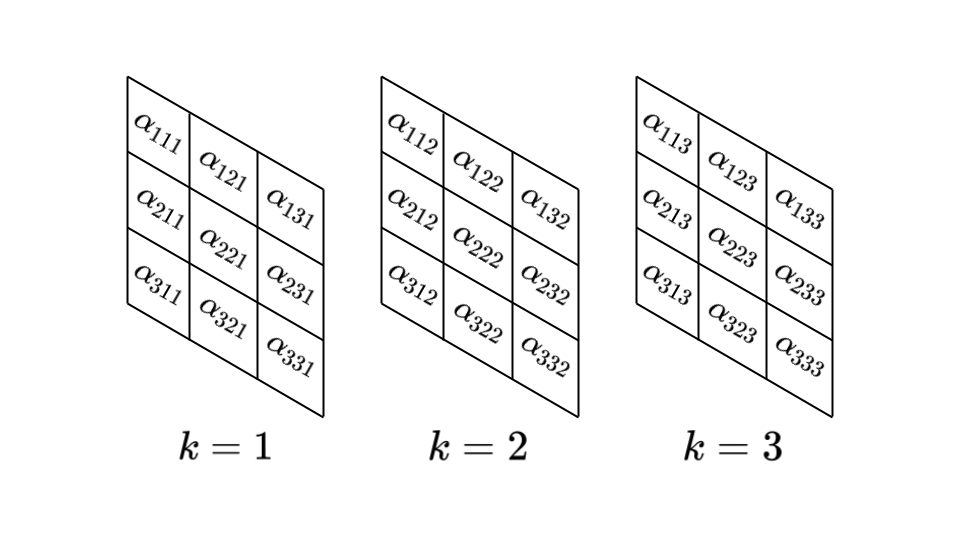
\includegraphics[width=\linewidth]{media/tridimensional_comp.png}
	\caption{Representación tridimensional completa de una cubriz con elementos $\alpha_{ijk}$.}
\end{figure}

\subsection{Producto.}

Bajo la definición ofrecida, el elemento $ijk$ de la cubriz $\Delta = (AB\Gamma)$ será igual al producto de la fila $i$ de $A$ por la columna $j$ de $B$ por la ``profundidad'' $k$ de $\Gamma$.

\begin{figure}[H]
	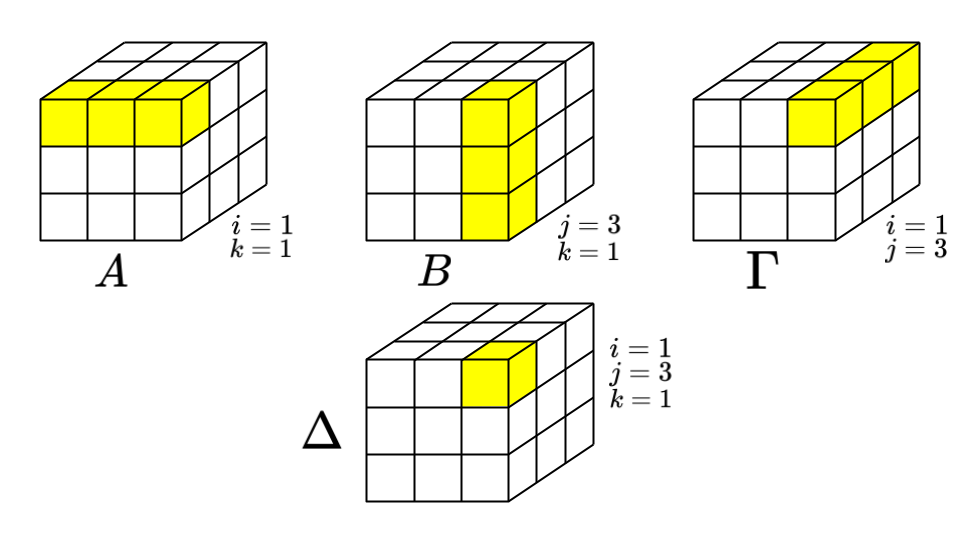
\includegraphics[width=\linewidth]{media/product.png}
	\caption{Representación tridimensional superficial del producto $\Delta = (AB\Gamma)$.}
\end{figure}

Esto explica las restricciones que marcan las dimensiones. En el proceso iterativo de la suma, es necesario que coincidan el número de columnas de $A$ ($n$), el número de filas de $B$ ($p$) y el número de ``profundidades'' de $\Gamma$ ($u$). Además, $\Delta$ no podrá tener más filas que $A$ ni que $\Gamma$ (de lo contrario, accederíamos a valores inexistentes), ni más columnas que $B$ o $\Gamma$, ni más ``profundidades'' que $A$ o $B$.
  % Cojonudo
\section{Notion of identity.} \label{identity}

The identity matrix $I$ is the one that satisfies that $AI = IA = A$. It's interesting to look for a similar notion in cubrices, however, we soon discover our expectations to be challenged.

\subsection{I's uniqueness.} \label{identity-unique}

Let $A, I \in M_{n} (\mathbb{K})$ such that $IIA = A$ (the reasoning works regardless of the product's order). We start from three assumptions:

\begin{itemize}
	\item No element from $A$ is zero.
	\item Elements from $I$ don't depend on ones from $A$.
	\item The identity cubrix $I$ is unique.
\end{itemize}

By definition:

$$A_{ijk} = (I \cdot I \cdot A)_{ijk} = \sum\limits_{l=1}^{n} I_{ilk} \cdot I_{ljk} \cdot A_{ijl}$$

Because we supposed that $I$ is independent from $A$, this expression can only yield $A_{ijk}$ from the sum's term $A_{ijl}$. In other words, $I_{ilk} I_{ljk} = \delta_{lk}$, where $\delta_{lk}$ is the $\delta{Kronecker delta}$, an expression we'll frequently use and which is equivalent to:

\begin{equation}
	\delta_{ab} =
	\begin{cases}
		1 & \text{if } a = b \\
		0 & \text{if } a \neq b
	\end{cases}
\end{equation}

According to the previous expressions we can derive a formula for $I_{ijk}$ by subtle manipulation of subindices. See $I_{ilk}$ and note that saying it is equal to $1$ if $l$ takes $k$'s value is equivalent to saying that it is equal to $1$ if its $j$ is equal to its $k$. In other words, $I_{ijk} = \delta_{jk}$. But applying the same reasoning over $I_{ljk}$ we get that $I_{ijk} = \delta_{ik}$. The only way to avoid this contradiction is to establish that $I_{ijk} = \delta_{jk} \delta_{ik}$, but this necessarily leaves out multiple elements of $A$. (See Appendix \ref{appendix-1} for a complete elaboration on the $M_2 (\mathbb{K})$ particular case if help is needed to clarify the patern).

At least one of our assumptions must be wrong, and it would be optimal for it to be the third one (on the identity's uniqueness).

\subsection{Identity as a pair.} \label{identity-pair}

We say that $I, J \in M_{n} (\mathbb{K})$ form an \textit{identity pair} if they satisfy that $AIJ = A$ (we'll later explore the influence on the order of factors). Once again, using the product's definition:

$$A_{ijk} = (AIJ)_{ijk} = \sum\limits_{l=1}^{n} A_{ilk} I_{ljk} J_{ijl}$$

This time, the conditions to be satisfied are:

\begin{itemize}
	\item $I_{ljk} = J_{ijl}^{-1}$ para $l = j$ y $I_{ljk} J_{ijl} = 0$ para $l \neq j$.
	\item $J_{ijl} = I_{ljk}^{-1}$ para $l = k$ y $J_{ijl} I_{ljk} = 0$ para $l \neq k$.
\end{itemize}

Any two cubrices that fulfill these conditions will be considered an \textit{identity pair}, and they will satisfy that $AIJ = A$. It's obvious that if $\mathbb{K}$ is a field, there will be infinitely many identity pairs, whereas if it's a commutative unitary ring, only the following ones will exist.

\subsection{The three Kroneckers.} \label{identity-kronecker}

For simplicity and standardization we can set all terms which must be the inverse of others to be equal to $1$, whereas we set all terms which must cancel out to be equal to $0$.

That is to say, for $(AIJ)_{ijk} = A_{ijk}$, then $I_{ljk} = J_{ijl} = \delta_{jl}$. With a reasoning very similar to the one in section \ref{identity-unique}, we can make these expressions independent from the $l$ subindex:

$$I_{ijk} = \delta_{ij}$$

Having in mind that the identity pair isn't commutative, it's easy to do something similar both for $I_2 A J_2$ and $I_3 J_3 A$ (commuting $I$ and $J$ won't produce new cubrices, but only commute their names). With $\Delta_{ab} = (\delta_{ab})$, we get that:

$$A = A \Delta_{ij} \Delta_{jk} = \Delta_{ij} A \Delta_{ik} = \Delta_{jk} \Delta_{ik} A$$

\newpage

With this we conclude that there exist three standard identity pairs grounded on the three Kroneckers. It isn't immediately obvious which pattern to take out from this result. In any case, it's intriguing to observe the cubrices drawn by each Kronecker. Let's take their complete three-dimensional representations.

\begin{figure}[H]
	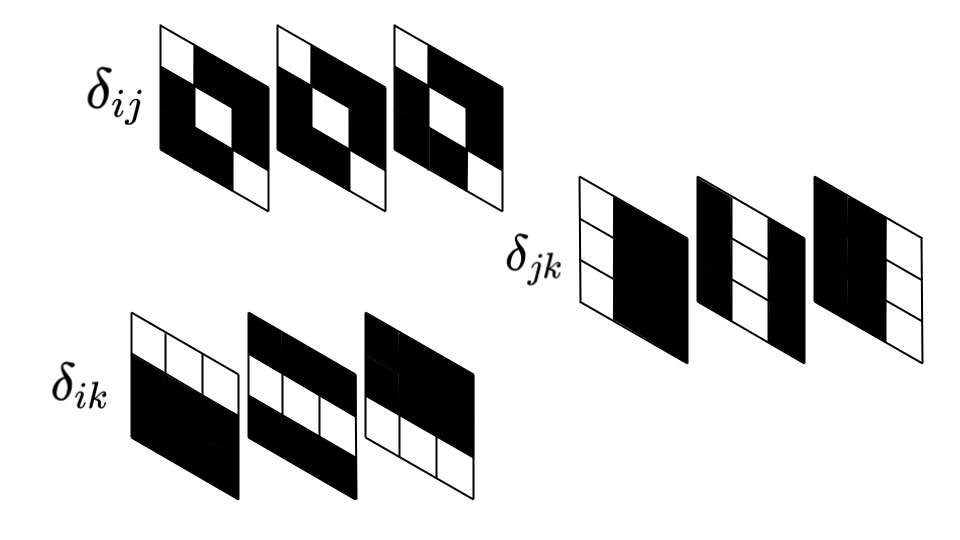
\includegraphics[width=\linewidth]{media/kroneckers.png}
	\caption{Complete three-dimensional representation of $\Delta_{ij}$, $\Delta{jk}$ y $\Delta{ik}$ (cells equal to $1$ in white and those equal to $0$ in black).}
\end{figure}

It can be useful to group and rename terms in the following way. If $I_{ijk} = 1$, then:

\begin{itemize}
	\item $A = A \Delta_{ij} I = A I \Delta_{jk}$.
	\item $A = \Delta_{ij} A I = I A \Delta_{ik}$.
	\item $A = \Delta_{jk} I A = I \Delta_{ik} A$.
\end{itemize}

\newpage
       % Otra expresión de la identidad.
\section{Noción de inversa.} \label{inverse}

\subsection{Par inversa.} \label{inverse-pair}

Al igual que antes, buscamos inspiración en el área de las matrices, donde la matriz inversa $A^{-1}$ a otra matriz $A$ es aquélla que satisface que ${A\cdot A^{-1} = A^{-1} \cdot A = I}$. Ya ha quedado en evidencia la multiplicidad de las cubrices identidad, así que hemos de esperar lo mismo para las cubrices inversas.

Decimos que $I$ y $J$ forman un \textit{par inversa} en $AIJ$ sobre $i, j$ si $(AIJ) = \Delta_{ij}$. Podemos afirmar lo mismo para pares en otros órdenes del producto ($IAJ$, $IJA$) y sobre otras cubrices kronecker ($\Delta_{jk}$, $\Delta_{ik}$). Nótese que la conmutatividad no está asegurada.

\subsection{Todos los pares inversas.} \label{inverse-all-pairs}

Tras un desarrollo algo repetitivo (ver Apéndice \ref{appendix-3}), recogeremos en la siguiente tabla todos los pares inversa no redundantes existentes.

\bgroup
\begin{table}[H] 
\centering
\captionsetup{labelformat=empty}
\caption{(Tabla 1) Pares inversa.}
\label{tabla-explicita}
\def\arraystretch{1.5}%  1 is the default, change whatever you need
\begin{tabular}{|c|c|c|c|} 
	\hline
	& $\Delta_{ij}$ & $\Delta_{jk}$ & $\Delta_{ik}$ \\
	\hline

	$AIJ$
	& \begin{tabular}{c} $I_{ijk} = \delta_{ij} A_{ijk}^{-1}$ \\ $J_{ijk} = \delta_{ij}$ \end{tabular}
	& \begin{tabular}{c} $I_{ijk} = \delta_{jk}$ \\ $J_{ijk} = \delta_{jk} A_{ijk}^{-1}$ \end{tabular}
	& \begin{tabular}{c} $I_{ijk} = \delta_{ik} A_{kkk}^{-1}$ \\ $J_{ijk} = \delta_{ik}$ \end{tabular} \\
	\hline

	$IAJ$
	& \begin{tabular}{c} $I_{ijk} = \delta_{ij} A_{ijk}^{-1}$ \\ $J_{ijk} = \delta_{ij}$ \end{tabular}
	& \begin{tabular}{c} $I_{ijk} = \delta_{jk} A_{jjj}^{-1}$ \\ $J_{ijk} = \delta_{jk}$ \end{tabular}
	& \begin{tabular}{c} $I_{ijk} = \delta_{ik}$ \\ $J_{ijk} = \delta_{ik} A_{ijk}^{-1}$ \end{tabular} \\
	\hline

	$IJA$
	& \begin{tabular}{c} $I_{ijk} = \delta_{ij} A_{iii}^{-1}$ \\ $J_{ijk} = \delta_{ij}$ \end{tabular}
	& \begin{tabular}{c} $I_{ijk} = \delta_{jk} A_{ijk}^{-1}$ \\ $J_{ijk} = \delta_{jk}$ \end{tabular}
	& \begin{tabular}{c} $I_{ijk} = \delta_{ik}$ \\ $J_{ijk} = \delta_{ik} A_{ijk}^{-1}$ \end{tabular} \\
	\hline
\end{tabular}
\end{table}
\egroup

Es fácil notar que con unos simples cambios de nombre podemos obtener un resultado mucho más limpio (ver Apéndice \ref{appendix-4}). Sea $(A^{-1})_{ijk} = (A_{ijk})^{-1}$ y $\Delta = (\delta_{ij}\delta_{jk})$. Podemos repartir sus productos con $A$ en distintas columnas según la kronecker que resulte del mismo.

\bgroup
\begin{table}[H]
\centering
\captionsetup{labelformat=empty}
\caption{(Tabla 2) Pares inversa simplificados.}
\label{tabla-simplificada}
\def\arraystretch{1.5}%  1 is the default, change whatever you need
\begin{tabular}{|c|c|c|c|} 
	\hline
	$\Delta_{ij}$ & $\Delta_{jk}$ & $\Delta_{ik}$ \\
	\hline
	\begin{tabular}{c} $(A \cdot A^{-1} \cdot \Delta)$ \\ $(A^{-1} \cdot A \cdot \Delta)$ \end{tabular} &
	\begin{tabular}{c} $(A \cdot \Delta \cdot A^{-1})$ \\ $(A^{-1} \cdot \Delta \cdot A)$ \end{tabular} &
	\begin{tabular}{c} $(\Delta \cdot A \cdot A^{-1})$ \\ $(\Delta \cdot A^{-1} \cdot A)$ \end{tabular} \\
	\hline
\end{tabular}
\end{table}
\egroup

Nótese la exclusión de la diagonal positiva de la primera tabla presentada. Aquéllas expresiones no pueden ser transformadas en términos tan limpios. Si bien podríamos afirmar que $((\delta_{ab} A^{-1}_{aaa}, (\delta_{ab}))$ constituye un par inversa para esos ordenes, consideramos que la belleza ha de primar sobre la completitud.

Analizando la última tabla, parece evidente que conmutar $A$ con $A^{-1}$ no altera el resultado. En otras palabras: es la posición de $\Delta$ la que determina qué cubriz Kronecker nacerá del producto. Por ejemplo, $\Delta_{jk}$ es producida cuando $\Delta$ ocupa la segunda posición. Esto tiene cierto sentido intuitivo, ya que en esta posición del producto, su subíndice $i$ se ve sustituído por el iterador $l$ del sumatorio, dejando como componentes restantes solo a $j$ y a $k$.
         % Reescribir un poco
\section{Programatic implementation.}

The study of this mathematical concept becomes tedious without computational assistance, so it'll be necessary to develop the tools that make it possible.

We offer the following GitHub repository created along this document: \href{https://github.com/erikucenik/cubrices}{https://github.com/erikucenik/cubrices}.

In addition, we include another repository which contains the most up-to-date version of this article: \href{https://github.com/erikucenik/cubrices-paper}{https://github.com/erikucenik/cubrices-paper}.
   % Cojonudo
\section{Conclusion.}

After this analysis we discover that cubrices conform a truly interesting and mysterious set. Contrary to what one might have thought, this algebra isn't backward compatible with two-dimensional matrices, although it's true that the underlying sets actually are.

We have left out many topics of vital importance which could be of interest to future investigations. Notions like the ``determinant'', the ``range'' or a definition of equality among cubrices which could make them backward compatible with matrices.

We hope that this document encourages the curiosity upon this algebra on the reader.
       % Cojonudo

\newpage

\counterwithin*{equation}{section}
\counterwithin*{equation}{subsection}
\counterwithin*{equation}{subsubsection}

\appendix
\section{Apéndice} \label{appendix}

\subsection{Desarrollo completo del producto por una hipotética cubriz identidad única en $M_2 (\mathbb{K})$.} \label{appendix-1}

La expresión $A = IIA$ puede ser desarrollada por la definición del producto cubricial:

\begin{equation}
A_{111} = I_{111} I_{111} A_{111} + I_{121} I_{211} A_{112}
\end{equation}

\begin{equation}
A_{112} = I_{112} I_{112} A_{111} + I_{122} I_{212} A_{112}
\end{equation}

\begin{equation}
A_{121} = I_{111} I_{121} A_{121} + I_{121} I_{221} A_{122}
\end{equation}

\begin{equation}
A_{122} = I_{112} I_{122} A_{121} + I_{122} I_{222} A_{122}
\end{equation}

\begin{equation}
A_{211} = I_{211} I_{111} A_{211} + I_{221} I_{211} A_{212}
\end{equation}

\begin{equation}
A_{212} = I_{212} I_{112} A_{211} + I_{222} I_{212} A_{212}
\end{equation}

\begin{equation}
A_{221} = I_{211} I_{121} A_{221} + I_{221} I_{221} A_{222}
\end{equation}

\begin{equation}
A_{222} = I_{212} I_{122} A_{221} + I_{222} I_{222} A_{222}
\end{equation}

En base a ese sistema derivamos lo siguiente:

\begin{enumerate}[(a)]
	\item Por $(1) \Rightarrow I_{111} = 1$.
	\item Por $(8) \Rightarrow I_{222} = 1$.
	\item Por $(3)$ y $(a) \Rightarrow I_{121} = 1$.
	\item Por $(3)$ y $(c) \Rightarrow I_{221} = 0$.
	\item Por $(6)$ y $(b) \Rightarrow I_{212} = 1$.
	\item Por $(2)$ y $(e) \Rightarrow I_{122} = 1$.
\end{enumerate}

Por $(8)$, o $I_{212}$ o $I_{122}$ deben ser $0$, pero por $(e)$ y $(f)$, $I_{212} = I_{122} = 1 \neq 0$. Surge la misma contradicción al probar con $IAI$ y $AII$.

\subsection{Desarrollo completo del producto por un par identidad en $M_2 (\mathbb{K})$.} \label{appendix-2}

\begin{equation}
A_{111} = A_{111} I_{111} J_{111} + A_{121} I_{211} J_{112}
\end{equation}

\begin{equation}
A_{112} = A_{112} I_{112} J_{111} + A_{122} I_{212} J_{112}
\end{equation}

\begin{equation}
A_{121} = A_{111} I_{121} J_{121} + A_{121} I_{221} J_{122}
\end{equation}

\begin{equation}
A_{122} = A_{112} I_{122} J_{121} + A_{122} I_{222} J_{122}
\end{equation}

\begin{equation}
A_{211} = A_{211} I_{111} J_{211} + A_{221} I_{211} J_{212}
\end{equation}

\begin{equation}
A_{212} = A_{212} I_{112} J_{211} + A_{222} I_{212} J_{212}
\end{equation}

\begin{equation}
A_{221} = A_{211} I_{121} J_{221} + A_{221} I_{221} J_{222}
\end{equation}

\begin{equation}
A_{222} = A_{212} I_{122} J_{221} + A_{222} I_{222} J_{222}
\end{equation}

De manera análoga, derivamos que:

\begin{enumerate}[(a)]
	\item Por $(1) \Rightarrow I_{111} \neq 0 \neq J_{111}$ y $I_{111} = J_{111}^{-1}$.
	\item Por $(8) \Rightarrow I_{222} \neq 0 \neq J_{222}$ y $I_{222} = J_{222}^{-1}$.
	\item Por $(2)$ y $(a) \Rightarrow I_{112} = J_{111}^{-1} = I_{111} \neq 0$.
	\item Por $(6)$ y $(c) \Rightarrow I_{112} = J_{211}^{-1} \neq 0 \Rightarrow J_{211} \neq 0$.
	\item Por $(5)$ y $(d) \Rightarrow J_{211} = I_{111}^{-1} = J_{111}$.
	\item Por $(7)$ y $(b) \Rightarrow I_{221} = J_{222}^{-1} \neq 0$.
	\item Por $(3)$, $(4)$ y $(f) \Rightarrow J_{122} = I_{221}^{-1} = I_{222}^{-1} = J_{222}^{-1}$.
	\item Por $(g)$ y $(b) \Rightarrow I_{222} = J_{222}^{-1} = I_{222}^{-1} \Rightarrow I_{222}^2 = 1 \Rightarrow I_{222} = 1 = J_{222}$.
\end{enumerate}

\newpage

Recapitulando:

\begin{itemize}
	\item $I_{221} = J_{122} = I_{222} = J_{222} = 1$.
	\item $J_{211}^{-1} = I_{111} = J_{111}^{-1} = I_{112}$.
	\item El resto de términos:

	\begin{itemize}
		\item $I_{211} J_{112} = 0$.
		\item $I_{212} J_{112} = 0$.
		\item $I_{121} J_{121} = 0$.
		\item $I_{122} J_{121} = 0$.
		\item $I_{211} J_{212} = 0$.
		\item $I_{212} J_{212} = 0$.
		\item $I_{121} J_{221} = 0$.
		\item $I_{122} J_{221} = 0$.
	\end{itemize}
\end{itemize}

Por cuestiones de estandarización, podemos asumir que los elementos que no se anulen con otros serán iguales a $1$, mientras que aquéllos que sí se anulen, serán $0$.

\begin{itemize}
	\item $1 = I_{221} = J_{122} = I_{222} = J_{222} = J_{211}^{-1} = I_{111} = J_{111}^{-1} = I_{112}$.
	\item $0 = I_{211} = J_{112} = I_{212} = I_{121} = J_{121} = I_{122} = J_{212} = J_{221}$.
\end{itemize}

Vemos que siempre se cumple que:

\begin{itemize}
	\item Si $j = 1 \rightarrow I_{1jk} = J_{ij1} = 1$ y $I_{2jk} = J_{ij2} = 0$.
	\item Si $j = 2 \rightarrow I_{1jk} = J_{ij1} = 0$ y $I_{2jk} = J_{ij2} = 1$.
\end{itemize}

El patrón se vuelve trivial si vemos qué ocurre con una cubriz $3 \times 3 \times 3$:

$$(AIJ)_{ijk} = A_{i1k} I_{1jk} J_{ij1} + A_{i2k} I_{2jk} J_{ij2} + A_{i3k} I_{3jk} J_{ij3}$$

\begin{itemize}
	\item Si $j = 1 \rightarrow I_{1jk} = J_{ij1} = 1$ y $I_{2jk} = J_{ij2} = 0$ y $I_{3jk} = J_{ij3} = 0$.
	\item Si $j = 2 \rightarrow I_{1jk} = J_{ij1} = 0$ y $I_{2jk} = J_{ij2} = 1$ y $I_{3jk} = J_{ij3} = 0$.
	\item Si $j = 3 \rightarrow I_{1jk} = J_{ij1} = 0$ y $I_{2jk} = J_{ij2} = 0$ y $I_{3jk} = J_{ij3} = 1$.
\end{itemize}

Es decir, para que $(AIJ)_{ijk} = A_{ijk}$, debe cumplirse que $I_{ljk} = J_{ijl} = \delta_{jl}$.

Como descubrimos en la sección \ref{identity-pair}, podemos manipular los subíndices hasta llegar a las tres Kronecker.

\subsection{Desarrollo completo de los pares inversa.} \label{appendix-3}

Dado $A$, nuestro objetivo es hallar sus pares inversa sobre dos componentes en cualquier orden de producto. Trataremos los productos que conmuten $I$ con $J$ como casos iguales (justificar $AIJ$ justificará también $AJI$), dado que el resultado de esto será solo conmutar los nombres de los valores.

\subsubsection{$AIJ$ sobre $i, j$.}

Por definición:

$$(AIJ)_{ijk} = \delta_{ij} = \sum\limits^{n}_{l = 1} A_{ilk} I_{ljk} J_{ijl}$$

Podemos explicar esta expresión en palabras: ``Si $i \neq j$, entonces $I_{ljk} J_{ijl} = 0$. Si $i = j$, y si además $l$ toma el valor de $j$, entonces $I_{ljk} = A^{-1}_{ilk}$ y $J_{ijl} = 1$''. Es vital notar que el hecho de que $l$ tome el valor de $j$ implica que el primer subíndice de $I_{ljk}$ también toma el valor de $j$. Esto equivale a que $i$ sea igual a $j$ (pero \textbf{solo} en el caso de $I$, pues en otros términos el iterador $l$ ocupará la posición de otro subíndice). Con esto en mente, expresar lo mismo utilizando deltas de Kronecker es automático:

$$I_{ijk} = \delta_{ij} \delta_{ij} A_{ijk}^{-1} = \delta_{ij} A_{ijk}^{-1}$$
$$J_{ijk} = \delta_{ij} \approx \delta_{ij} \delta_{jk}$$

En $I$, el primer $\delta_{ij}$ representa la condición que impone la delta de Kronecker a la que aspiramos a llegar, mientras que el segundo $\delta_{ij}$ representa la condición que impone el iterador $l$ pero expresada en términos de subíndices de $I$. Como es evidente, $\delta_{ij} \delta_{ij} = \delta_{ij}$.

En $J$, el término $\delta_{jk}$ representa la condición de ``...si $i = j$ pero $l$ no toma el valor de $j$...'' (lo que en $J$ equivale a que $k$ no tome el valor de $j$). Este término es innecesario, ya que solo se requiere la anulación del producto (y no de ambos factores), y esto ya se satisface gracias al $\delta_{ij}$ presente en $I$. Las condiciones impuestas sobre los valores de $I$ y $J$ quedan perfectamente representadas en el siguiente algoritmo:

\begin{lstlisting}[escapeinside={(*}{*)}]
Si i == j:
  Si l == j:
    (*$I_{ljk} = A_{ilk}^{-1}$*)
    (*$J_{ijl} = 1$*)
  Si no:
    (*$I_{ljk} J_{ijl} = 0$*)
Si no:
  (*$I_{ljk} J_{ijl} = 0$*)	
\end{lstlisting}

En este artículo omitimos la inclusión del segundo factor, tanto por motivos estéticos como prácticos (véase \ref{appendix-4}).

\subsubsection{$AIJ$ sobre $j, k$.}

El proceso es casi idéntico al anterior, pero conmutaremos $I$ con $J$ (los valores inversos pasarán a estar en $J$, y los neutros en $I$). La necesidad de hacer esto yace en el deseo de coordinar los subíndices de $I$ y $J$ con el iterador de tal manera que obtengamos expresiones fácilmente maleables como $\delta_{jk} \delta_{jk}$.

\newpage

\subsubsection{$AIJ$ sobre $i, k$.}

Este caso requiere algo de atención. Sea $a = i = k$ (en caso de que $i \neq k$, el producto de $I_{ijk}$ y $J_{ijk}$ será cero):

$$\delta_{aa} = 1 = \sum\limits_{l = 1}^{n} A_{ala} I_{lja} J_{ajl}$$

Hasta ahora, $I_{ijk}$ siempre había dependido del inverso de $A_{ijk}$, sin embargo este caso rompe esa relación. Es por eso que tenemos que buscar otro criterio para no anular a $I$ y a $J$. Nuevamente por una mezcla de motivos estéticos y proceso de eliminación, establecemos lo siguiente: que cuando los índices de $I$ y $J$ sean iguales, su producto con $A_{ijk}$ dará $1$ (y cuando no, $0$).

Es fácil descubrir que los subíndices de $I$ y $J$ serán iguales cuando $l$ tome el valor de $a$. Es decir:

$$I_{aja} = A_{aaa}^{-1}$$
$$J_{aja} = 1$$

O expresado con $i$, $j$ y $k$:

$$I_{ijk} = \delta_{ik} A_{iii}^{-1} = \delta_{ik} A_{kkk}^{-1}$$
$$J_{ijk} = \delta_{ik}$$

\subsubsection{Et cetera.}

Hemos trabajado con $AIJ$, pero podríamos haber hecho los mismos procedimientos sobre $IAJ$ e $IJA$. Todos los casos se pueden resolver de forma análoga con uno de los tres métodos anteriores, y el resultado final es la Tabla \ref{tabla-explicita} de la sección \ref{inverse-all-pairs}.

\subsection{Simplificación de los pares inversa.} \label{appendix-4}

Las expresiones de los pares inversa pueden ser simplificadas con bastante éxito tan solo reordenando algunos términos.

Como primer y único ejemplo usaremos el caso de $IJA$ sobre $i, k$. Según la Tabla \ref{tabla-explicita}:

$$I_{ijk} = \delta_{ik}$$
$$J_{ijk} = \delta_{ik} A_{ijk}^{-1}$$

Insertando eso en la definición del producto:

$$(IJA)_{ijk} = (\delta_{ik})_{ilk} \cdot (\delta_{ik} A_{ijk}^{-1})_{ljk} \cdot A$$

Y sustituyendo los subíndices:

$$(IJA)_{ijk} = (\delta_{ik}) \cdot (\delta_{lk} A_{ljk}^{-1}) \cdot A$$

\newpage

Gracias a que $\mathbb{K}$ es asociativo y conmutativo, podemos reescribir esta expresión tal que:

$$(IJA)_{ijk} = (\delta_{ik} \delta_{lk}) \cdot A_{ljk}^{-1} \cdot A$$

Y esto es equivalente a tener otro par inversa $(I', J')$ donde:

$$I'_{ijk} = \delta_{ik} \delta_{jk}$$
$$J'_{ijk} = (A_{ijk})^{-1}$$

($l$ se sustituiría en $j$ para $I$ y en $i$ para $J$).

Para dar algo de sentido semántico a este par inversa, podemos llamar $\Delta$ a $I'$ y $A^{-1}$ a $J'$.

La misma receta es aplicable al resto de casos (excluyendo aquéllos de la diagonal positiva en la Tabla \ref{tabla-explicita} de la sección \ref{inverse-all-pairs}), y produce la Tabla \ref{tabla-simplificada} de la sección \ref{inverse-all-pairs}.


\end{document}
